% =====================================================================
%  FacultyConnect: An Academic Collaboration Hub  --  Project Report
%  IEEE conference format (IEEEtran). Overleaf: Upload Project -> this zip
%  Compiler: pdfLaTeX
% =====================================================================
\documentclass[conference]{IEEEtran}
\IEEEoverridecommandlockouts

\usepackage{cite}
\usepackage{amsmath,amssymb}
\usepackage{algorithm}
\usepackage{algpseudocode}
\usepackage{graphicx}
\usepackage{xcolor}
\usepackage{booktabs}
\usepackage{tabularx}
\usepackage{array}
\usepackage{enumitem}
\usepackage{tikz}
\usetikzlibrary{positioning,arrows.meta,shapes.geometric,shapes.multipart,fit,backgrounds}
\usepackage{pgfgantt}
\usepackage[hidelinks]{hyperref}
\usepackage{url}

\definecolor{brand}{HTML}{5A4AD1}
\definecolor{coral}{HTML}{D9533D}
\definecolor{mint}{HTML}{1F9E74}
\setlist{nosep,leftmargin=1.2em}
\newcolumntype{Y}{>{\raggedright\arraybackslash}X}
\tikzset{
  box/.style={draw=brand,rounded corners=2pt,fill=brand!6,align=center,font=\scriptsize,inner sep=3pt,minimum height=6.5mm},
  ext/.style={draw=coral,rounded corners=2pt,fill=coral!7,align=center,font=\scriptsize,inner sep=3pt,minimum height=6.5mm},
  store/.style={draw=mint,fill=mint!7,align=center,font=\scriptsize,inner sep=3pt,minimum height=6mm},
  arr/.style={-{Latex[length=1.6mm]},semithick,draw=black!65},
  lbl/.style={font=\tiny,fill=white,inner sep=1pt}
}
% one screenshot per figure, full column width
\newcommand{\shot}[3]{\begin{figure}[!t]\centering\includegraphics[width=\columnwidth]{figures/#1}\caption{#2}\label{#3}\end{figure}}

\begin{document}

\title{FacultyConnect: An Academic Collaboration Hub}

\author{
\IEEEauthorblockN{Vani Tripathi}
\IEEEauthorblockA{Roll No. 1024160073\\
vtripathi\_be24@thapar.edu}
\and
\IEEEauthorblockN{Agrim Mittal}
\IEEEauthorblockA{Roll No. 1024160068\\
Amittal3\_be24@thapar.edu}
\and
\IEEEauthorblockN{Shriyam Bhardwaj}
\IEEEauthorblockA{Roll No. 1024160062\\
sbhardwaj1\_be24@thapar.edu}
}

\maketitle

\begin{abstract}
FacultyConnect is a web platform that helps students find the right faculty member and everything that faculty member has shared, in one place. It provides a searchable faculty directory, detailed profiles, a single date-wise \emph{All work} timeline of uploaded material, assignments with progress tracking, an interactive question bank, structured messaging and an AI-assisted faculty recommender. The system supports Student, Faculty and Administrator roles. This report presents the requirements, design, implementation, interface, testing and results of the project. A working prototype is deployed at \url{https://faculty-connect-mu.vercel.app/}.
\end{abstract}

\begin{IEEEkeywords}
FacultyConnect, faculty discovery, academic collaboration, timeline, recommendation, web application
\end{IEEEkeywords}

% =====================================================================
\section{Introduction}
Students need faculty guidance for projects, research, doubts and course material, but information about faculty expertise, openings and shared resources is scattered across department pages, e-mail and messaging groups. Faculty, in turn, have no single place to publish material and receive organised requests. FacultyConnect brings students, faculty, resources and opportunities together on one platform.

\textbf{Objectives:}
\begin{enumerate}
  \item Help students find suitable faculty through search, filters and recommendations.
  \item Keep each faculty member's material in one chronological timeline.
  \item Track assignments, videos watched and questions attempted.
  \item Provide structured student--faculty messaging.
  \item Let faculty publish material, assignments and questions in seconds.
\end{enumerate}

% =====================================================================
\section{Existing Systems}
Table~\ref{tab:compare} compares FacultyConnect with the channels students use today.

\begin{table}[!t]
\caption{Comparison with Existing Approaches}
\label{tab:compare}
\centering\scriptsize
\setlength{\tabcolsep}{3pt}
\begin{tabular}{@{}lccccc@{}}
\toprule
\textbf{Capability} & \textbf{Dept.} & \textbf{LMS} & \textbf{Researcher} & \textbf{Chat} & \textbf{Faculty-}\\
 & \textbf{site} & & \textbf{DB} & \textbf{groups} & \textbf{Connect}\\
\midrule
Search by research area   & -- & -- & \checkmark & -- & \checkmark\\
Faculty-wise resources    & -- & partial & -- & partial & \checkmark\\
Dated, ordered material   & -- & \checkmark & -- & -- & \checkmark\\
Assignments \& progress   & -- & \checkmark & -- & -- & \checkmark\\
Question bank             & -- & partial & -- & -- & \checkmark\\
Structured requests       & -- & -- & -- & -- & \checkmark\\
Faculty recommendation    & -- & -- & partial & -- & \checkmark\\
\bottomrule
\end{tabular}
\end{table}

% =====================================================================
\section{Proposed System}
\subsection{User Roles}
\begin{table}[!t]
\caption{User Roles and Permissions}
\label{tab:roles}
\centering\scriptsize
\begin{tabularx}{\columnwidth}{@{}l Y@{}}
\toprule
\textbf{Role} & \textbf{Can do}\\
\midrule
Student & Search faculty, view profiles and timelines, get recommendations, attempt question bank, mark assignments done, send requests, use helpdesk\\
Faculty & All student views, plus add work to timeline, add questions, read requests, view dashboard statistics\\
Administrator & Manage users, departments, faculty records and content approvals (planned)\\
\bottomrule
\end{tabularx}
\end{table}

\subsection{Key Features}
\begin{itemize}
  \item \textbf{Faculty directory} with department filters and global search.
  \item \textbf{Profiles} with nine tabs: About, All work, Research, Publications, Teaching, Assignments, Question bank, Students, Contact.
  \item \textbf{All work timeline}: every upload, assignment, lecture unit and question in one list, newest first, grouped by month.
  \item \textbf{Assignments} with automatic open/closed status.
  \item \textbf{Question bank} with instant MCQ feedback.
  \item \textbf{Messaging} with reason tags and live notification.
  \item \textbf{AI recommender} and \textbf{helpdesk chatbot}.
\end{itemize}

% =====================================================================
\section{Requirements}

\begin{table}[!t]
\caption{Functional Requirements}
\label{tab:fr}
\centering\scriptsize
\begin{tabularx}{\columnwidth}{@{}l Y l@{}}
\toprule
\textbf{ID} & \textbf{Requirement} & \textbf{Status}\\
\midrule
FR1 & Role-based sign-in & Done\\
FR2 & Search and filter faculty & Done\\
FR3 & Faculty profile with nine tabs & Done\\
FR4 & Add work item with date, type, course, file & Done\\
FR5 & Unified timeline grouped by month, type filters & Done\\
FR6 & Assignment completion and progress tracking & Done\\
FR7 & MCQ attempt with instant feedback & Done\\
FR8 & Faculty adds questions to bank & Done\\
FR9 & Structured messages with notification & Done\\
FR10 & Faculty recommendation (top 3 with reason) & Done\\
FR11 & Helpdesk chatbot & Done\\
FR12 & Administrator console & Planned\\
\bottomrule
\end{tabularx}
\end{table}

\begin{table}[!t]
\caption{Non-Functional Requirements}
\label{tab:nfr}
\centering\scriptsize
\begin{tabularx}{\columnwidth}{@{}l Y@{}}
\toprule
\textbf{Attribute} & \textbf{Target}\\
\midrule
Performance & Page loads in under 2\,s; view switch under 300\,ms\\
Availability & Works without database or AI by falling back to local storage\\
Usability & Responsive from 360\,px width; tasks in $\le$3 clicks\\
Security & All user text escaped before display; JWT in production\\
Portability & Chrome, Edge, Firefox, Safari; static hosting\\
\bottomrule
\end{tabularx}
\end{table}

Tables~\ref{tab:fr} and~\ref{tab:nfr} list the requirements. Eleven of twelve functional requirements are implemented in the prototype.

% =====================================================================
\section{System Design}

\subsection{Architecture}
Fig.~\ref{fig:arch} shows the proposed production architecture (React.js front end, Node.js/Express.js API, MongoDB/PostgreSQL). The current prototype is a single-page app (HTML, CSS, JavaScript) with an optional shared database and AI service (Fig.~\ref{fig:proto}).

\begin{figure*}[!t]
\centering
\resizebox{0.72\textwidth}{!}{%
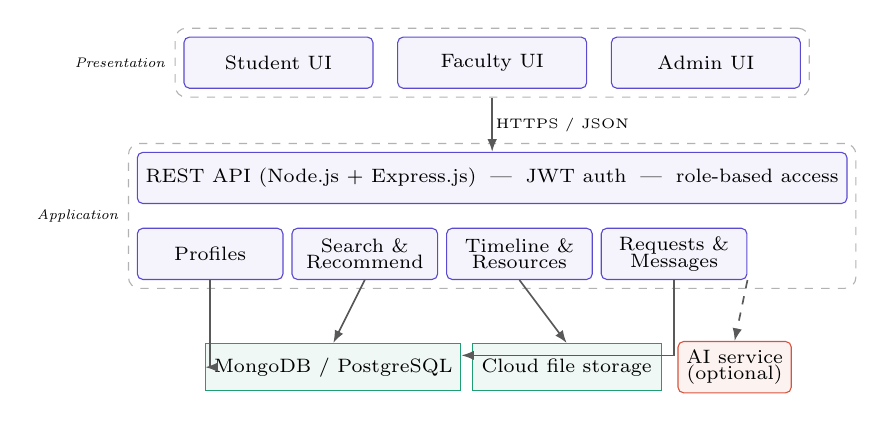
\begin{tikzpicture}[node distance=4mm and 3mm]
\node[box,minimum width=2.4cm] (s) {Student UI};
\node[box,right=of s,minimum width=2.4cm] (f) {Faculty UI};
\node[box,right=of f,minimum width=2.4cm] (a) {Admin UI};
\node[draw=black!30,dashed,rounded corners,fit=(s)(f)(a),inner sep=3pt,label={[font=\tiny\itshape]left:Presentation}] (pt) {};
\node[box,below=8mm of f,minimum width=7.9cm] (api) {REST API (Node.js + Express.js) \;|\; JWT auth \;|\; role-based access};
\node[box,below=3mm of api.south west,anchor=north west,minimum width=1.85cm] (m1) {Profiles};
\node[box,right=1mm of m1,minimum width=1.85cm] (m2) {Search \&\\[-2pt]Recommend};
\node[box,right=1mm of m2,minimum width=1.85cm] (m3) {Timeline \&\\[-2pt]Resources};
\node[box,right=1mm of m3,minimum width=1.85cm] (m4) {Requests \&\\[-2pt]Messages};
\node[draw=black!30,dashed,rounded corners,fit=(api)(m1)(m4),inner sep=3pt,label={[font=\tiny\itshape]left:Application}] (at) {};
\node[store,below=8mm of m2,minimum width=2.6cm,xshift=-4mm] (db) {MongoDB / PostgreSQL};
\node[store,below=8mm of m3,minimum width=2.4cm,xshift=6mm] (fs) {Cloud file storage};
\node[ext,right=2mm of fs,minimum width=1.4cm] (ai) {AI service\\[-2pt](optional)};
\draw[arr] (pt.south) -- node[lbl,right]{HTTPS / JSON} (api.north);
\draw[arr] (m2.south) -- (db.north); \draw[arr] (m1.south) |- (db.west);
\draw[arr] (m3.south) -- (fs.north); \draw[arr] (m4.south) |- ([yshift=1.5mm]db.east);
\draw[arr,dashed] (m4.south east) -- (ai.north);
\end{tikzpicture}}
\caption{Proposed three-tier architecture.}
\label{fig:arch}
\end{figure*}

\begin{figure}[!t]
\centering
\resizebox{0.86\columnwidth}{!}{%
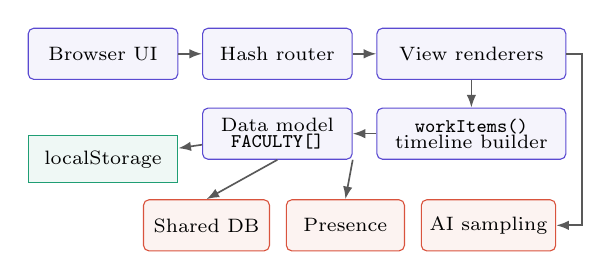
\begin{tikzpicture}[node distance=3.5mm and 3mm]
\node[box,minimum width=1.9cm] (ui) {Browser UI};
\node[box,right=of ui,minimum width=1.9cm] (rt) {Hash router};
\node[box,right=of rt,minimum width=2.4cm] (vw) {View renderers};
\node[box,below=of rt,minimum width=1.9cm] (dm) {Data model\\[-2pt]\texttt{FACULTY[]}};
\node[box,below=of vw,minimum width=2.4cm] (tl) {\texttt{workItems()}\\[-2pt]timeline builder};
\node[store,below=7mm of ui,minimum width=1.9cm] (ls) {localStorage};
\node[ext,below=5mm of dm,minimum width=1.6cm,xshift=-9mm] (db) {Shared DB};
\node[ext,right=2mm of db,minimum width=1.5cm] (pr) {Presence};
\node[ext,right=2mm of pr,minimum width=1.6cm] (ai) {AI sampling};
\draw[arr] (ui)--(rt); \draw[arr] (rt)--(vw); \draw[arr] (vw)--(tl); \draw[arr] (tl)--(dm);
\draw[arr] (dm)--(ls); \draw[arr] (dm.south)--(db.north); \draw[arr] (dm.south east)--(pr.north);
\draw[arr] (vw.east) -- ++(2mm,0) |- (ai.east);
\end{tikzpicture}}
\caption{Prototype architecture; red parts are optional with automatic fallback.}
\label{fig:proto}
\end{figure}

\subsection{UML and Data Models}
Figs.~\ref{fig:usecase}--\ref{fig:seq} show the use-case, data-flow, entity--relationship and sequence diagrams.

\begin{figure*}[!t]
\centering
\resizebox{0.78\textwidth}{!}{%
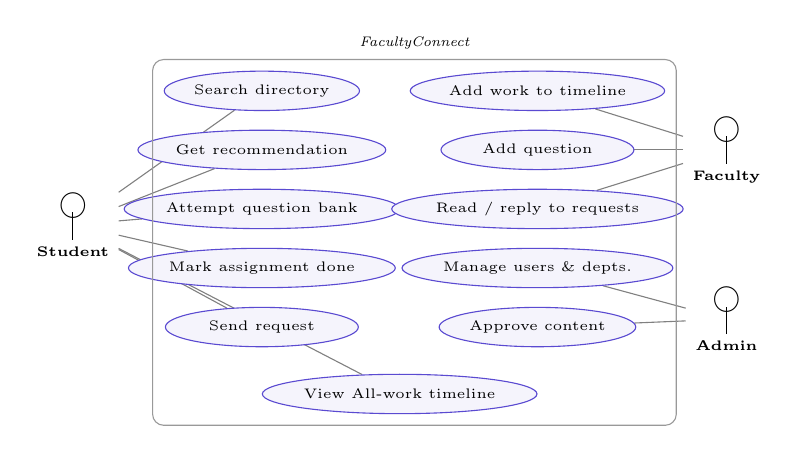
\begin{tikzpicture}[font=\scriptsize,
  uc/.style={ellipse,draw=brand,fill=brand!6,minimum width=2.45cm,minimum height=5mm,inner sep=0.5pt,font=\tiny},
  actor/.style={align=center,font=\tiny\bfseries}]
\node[actor] (stu) at (0,0.3) {\normalsize$\bigcirc$\\[-3pt]\rule{0.4pt}{3.5mm}\\Student};
\node[actor] (fac) at (8.3,1.25) {\normalsize$\bigcirc$\\[-3pt]\rule{0.4pt}{3.5mm}\\Faculty};
\node[actor] (adm) at (8.3,-0.9) {\normalsize$\bigcirc$\\[-3pt]\rule{0.4pt}{3.5mm}\\Admin};
\node[uc] (u1) at (2.4,2.0) {Search directory};
\node[uc] (u2) at (2.4,1.25) {Get recommendation};
\node[uc] (u3) at (2.4,0.5) {Attempt question bank};
\node[uc] (u4) at (2.4,-0.25) {Mark assignment done};
\node[uc] (u5) at (2.4,-1.0) {Send request};
\node[uc] (u0) at (4.15,-1.85) {View All-work timeline};
\node[uc] (u6) at (5.9,2.0) {Add work to timeline};
\node[uc] (u7) at (5.9,1.25) {Add question};
\node[uc] (u8) at (5.9,0.5) {Read / reply to requests};
\node[uc] (u9) at (5.9,-0.25) {Manage users \& depts.};
\node[uc] (u10) at (5.9,-1.0) {Approve content};
\node[draw=black!40,rounded corners,fit=(u1)(u0)(u6)(u10),inner sep=4pt,label={[font=\tiny\itshape]above:FacultyConnect}] {};
\begin{scope}[on background layer]
\foreach \u in {u1,u2,u3,u4,u5,u0} \draw[black!50] (stu)--(\u);
\foreach \u in {u6,u7,u8} \draw[black!50] (fac)--(\u);
\foreach \u in {u9,u10} \draw[black!50] (adm)--(\u);
\end{scope}
\end{tikzpicture}}
\caption{Use-case diagram.}
\label{fig:usecase}
\end{figure*}

\begin{figure}[!t]
\centering
\resizebox{\columnwidth}{!}{%
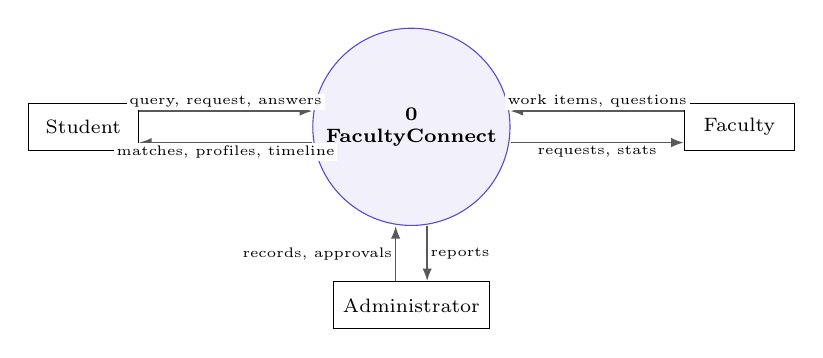
\begin{tikzpicture}[node distance=5mm]
\node[circle,draw=brand,fill=brand!8,minimum size=15mm,align=center,font=\scriptsize\bfseries] (p) {0\\FacultyConnect};
\node[draw,minimum width=1.4cm,minimum height=6mm,font=\scriptsize,left=2.2cm of p] (s) {Student};
\node[draw,minimum width=1.4cm,minimum height=6mm,font=\scriptsize,right=2.2cm of p] (f) {Faculty};
\node[draw,minimum width=1.4cm,minimum height=6mm,font=\scriptsize,below=7mm of p] (a) {Administrator};
\draw[arr] ([yshift=2mm]s.east) -- node[lbl,above]{query, request, answers} ([yshift=2mm]p.west);
\draw[arr] ([yshift=-2mm]p.west) -- node[lbl,below]{matches, profiles, timeline} ([yshift=-2mm]s.east);
\draw[arr] ([yshift=2mm]f.west) -- node[lbl,above]{work items, questions} ([yshift=2mm]p.east);
\draw[arr] ([yshift=-2mm]p.east) -- node[lbl,below]{requests, stats} ([yshift=-2mm]f.west);
\draw[arr] ([xshift=-2mm]a.north) -- node[lbl,left]{records, approvals} ([xshift=-2mm]p.south);
\draw[arr] ([xshift=2mm]p.south) -- node[lbl,right]{reports} ([xshift=2mm]a.north);
\end{tikzpicture}}
\caption{Level-0 data-flow diagram.}
\label{fig:dfd}
\end{figure}

\begin{figure}[!t]
\centering
\resizebox{\columnwidth}{!}{%
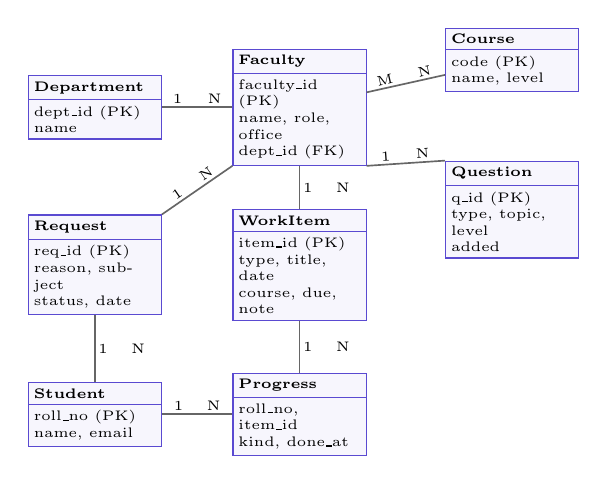
\begin{tikzpicture}[font=\tiny,
  ent/.style={rectangle split,rectangle split parts=2,draw=brand,fill=brand!5,font=\tiny,align=left,inner sep=2pt,text width=1.55cm},
  rel/.style={-,semithick,draw=black!60},
  card/.style={font=\tiny,inner sep=1pt}]
\node[ent] (dep) at (0,0) {\textbf{Department}\nodepart{second}dept\_id (PK)\\name};
\node[ent] (fac) at (2.6,0) {\textbf{Faculty}\nodepart{second}faculty\_id (PK)\\name, role, office\\dept\_id (FK)};
\node[ent] (crs) at (5.3,0.6) {\textbf{Course}\nodepart{second}code (PK)\\name, level};
\node[ent] (wi)  at (2.6,-2.0) {\textbf{WorkItem}\nodepart{second}item\_id (PK)\\type, title, date\\course, due, note};
\node[ent] (q)   at (5.3,-1.3) {\textbf{Question}\nodepart{second}q\_id (PK)\\type, topic, level\\added};
\node[ent] (req) at (0,-2.0) {\textbf{Request}\nodepart{second}req\_id (PK)\\reason, subject\\status, date};
\node[ent] (stu) at (0,-3.9) {\textbf{Student}\nodepart{second}roll\_no (PK)\\name, email};
\node[ent] (pg)  at (2.6,-3.9) {\textbf{Progress}\nodepart{second}roll\_no, item\_id\\kind, done\_at};
\draw[rel] (dep) -- node[card,above]{1 \quad N} (fac);
\draw[rel] (fac) -- node[card,above,sloped]{M \quad N} (crs);
\draw[rel] (fac) -- node[card,right]{1 \;\; N} (wi);
\draw[rel] (fac.south east) -- node[card,above,sloped]{1 \quad N} (q.north west);
\draw[rel] (fac.south west) -- node[card,above,sloped]{1 \;\; N} (req.north east);
\draw[rel] (stu) -- node[card,right]{1 \;\; N} (req);
\draw[rel] (stu) -- node[card,above]{1 \;\; N} (pg);
\draw[rel] (wi) -- node[card,right]{1 \;\; N} (pg);
\end{tikzpicture}}
\caption{Entity--relationship diagram.}
\label{fig:er}
\end{figure}

\begin{figure}[!t]
\centering
\resizebox{\columnwidth}{!}{%
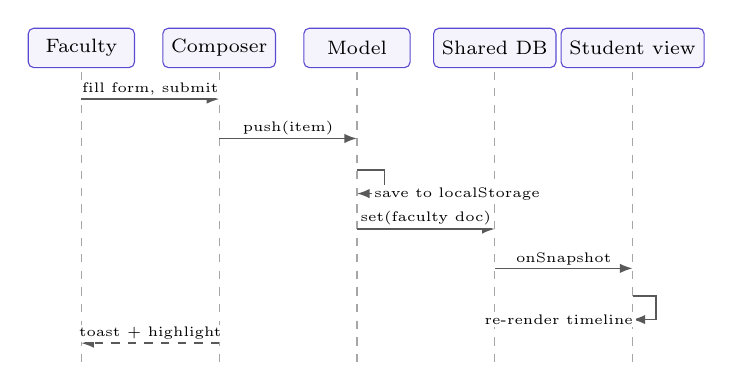
\begin{tikzpicture}[font=\tiny]
\foreach \x/\n/\t in {0/f/Faculty,1.75/ui/Composer,3.5/m/Model,5.25/db/Shared DB,7.0/v/Student view}{
  \node[box,minimum width=1.35cm,minimum height=5mm] (\n) at (\x,0) {\t};
  \draw[black!35,dashed] (\x,-0.3) -- (\x,-4.0);}
\def\msg#1#2#3#4{\draw[arr] (#1,#3) -- node[lbl,above]{#4} (#2,#3);}
\msg{0}{1.75}{-0.65}{fill form, submit}
\msg{1.75}{3.5}{-1.15}{push(item)}
\draw[arr] (3.5,-1.55) -- ++(0.35,0) -- ++(0,-0.3) -- node[lbl,right]{save to localStorage} (3.5,-1.85);
\msg{3.5}{5.25}{-2.3}{set(faculty doc)}
\msg{5.25}{7.0}{-2.8}{onSnapshot}
\draw[arr] (7.0,-3.15) -- ++(0.3,0) -- ++(0,-0.3) -- node[lbl,left,xshift=-1mm]{re-render timeline} (7.0,-3.45);
\draw[arr,dashed] (1.75,-3.75) -- node[lbl,above]{toast + highlight} (0,-3.75);
\end{tikzpicture}}
\caption{Sequence diagram: adding an item to the timeline.}
\label{fig:seq}
\end{figure}

% =====================================================================
\section{Implementation}

\begin{table}[!t]
\caption{Technology Stack}
\label{tab:stack}
\centering\scriptsize
\begin{tabularx}{\columnwidth}{@{}l Y Y@{}}
\toprule
\textbf{Layer} & \textbf{Proposed} & \textbf{Prototype}\\
\midrule
Frontend & React.js, Tailwind CSS & HTML5, CSS3, JavaScript\\
Backend & Node.js, Express.js & Client-side only\\
Database & MongoDB / PostgreSQL & Shared DB + localStorage\\
Auth & JWT & Simulated role picker\\
Search & Keyword overlap & Keyword overlap + optional AI\\
Hosting & Cloud PaaS & Vercel\\
Testing & Jest, Playwright & Playwright\\
\bottomrule
\end{tabularx}
\end{table}

\begin{table}[!t]
\caption{Modules}
\label{tab:modules}
\centering\scriptsize
\begin{tabularx}{\columnwidth}{@{}l Y@{}}
\toprule
\textbf{Module} & \textbf{What it does}\\
\midrule
Router & Maps URLs like \texttt{\#/faculty/id/work} to views\\
Directory & Search across name, department, research, publications\\
Profile & Renders the nine profile tabs\\
Timeline & Merges all shared items, sorts by date, groups by month\\
Assessment & Assignments status, MCQ checking, question authoring\\
Messaging & Contact form, faculty inbox, notification badge\\
Recommender & Ranks faculty for a free-text interest\\
\bottomrule
\end{tabularx}
\end{table}


\begin{table}[!t]
\caption{Data Dictionary: WorkItem}
\label{tab:dd}
\centering\scriptsize
\begin{tabularx}{\columnwidth}{@{}l l Y@{}}
\toprule
\textbf{Field} & \textbf{Type} & \textbf{Description}\\
\midrule
id & string & Unique item identifier\\
title & string & Item title shown in the timeline\\
type & enum & lecture, video, solutions, paper, project, assignment\\
course & string & Course code, e.g.\ CSE452 (optional)\\
date & date & Date shared; orders the timeline\\
due & date & Due date (assignments only)\\
note & string & Short note for students\\
fileName & string & Attached file name (optional)\\
views & integer & Number of times opened\\
\bottomrule
\end{tabularx}
\end{table}

\subsection{All Work Timeline}
Table~\ref{tab:dd} lists the fields of a work item. Previously, uploads were shown in a separate list. Now every item a faculty member shares is merged into one timeline (Algorithm~\ref{alg:timeline}). Faculty can also set an earlier date so older work appears in the correct month.

\begin{algorithm}[!t]
\caption{Build the All Work timeline}
\label{alg:timeline}
\small
\begin{algorithmic}[1]
\Require faculty $f$, filter $t$
\State $I \gets$ uploads $\cup$ assignments $\cup$ lectures $\cup$ questions of $f$
\State sort $I$ by date, newest first
\If{$t \neq$ all} \State keep only items of type $t$ \EndIf
\State group $I$ by (year, month)
\State \Return groups
\end{algorithmic}
\end{algorithm}

\subsection{Faculty Recommendation}
For query $q$ with words $W(q)$ and faculty research areas $R_f$:
\begin{equation}
s(f,q)=\max_{r\in R_f}\;\sum_{w\in W(q)} \mathbb{1}\left[w \in \mathrm{text}(r)\right]
\end{equation}
The top three faculty with $s>0$ are shown with the matching area as the reason. When AI is available, a language model ranks faculty instead.

% =====================================================================
\section{Prototype Screens}
Figs.~\ref{fig:big1}--\ref{fig:screens3} show the implemented screens. Table~\ref{tab:walk} walks through the main tasks for each role.

\begin{table}[!t]
\caption{User Walkthrough}
\label{tab:walk}
\centering\scriptsize
\begin{tabularx}{\columnwidth}{@{}l Y l@{}}
\toprule
\textbf{\#} & \textbf{Step} & \textbf{Screen}\\
\midrule
\multicolumn{3}{@{}l}{\textit{Student}}\\
1 & Sign in as Student & Fig.~\ref{fig:screens2}a\\
2 & See stats, feed and progress & Fig.~\ref{fig:big2}a\\
3 & Search or filter faculty & Fig.~\ref{fig:screens2}b\\
4 & Open a profile & Fig.~\ref{fig:big2}b\\
5 & Browse \emph{All work}, filter by type & Fig.~\ref{fig:big1}a\\
6 & Mark an assignment done & Fig.~\ref{fig:screens2}d\\
7 & Practise questions & Fig.~\ref{fig:screens2}e\\
8 & Get a faculty recommendation & Fig.~\ref{fig:screens2}f\\
9 & Send a request & Fig.~\ref{fig:screens2}g\\
\midrule
\multicolumn{3}{@{}l}{\textit{Faculty}}\\
1 & Sign in, choose own profile & Fig.~\ref{fig:screens2}a\\
2 & View dashboard statistics & Fig.~\ref{fig:screens2}h\\
3 & Add work (title, type, course, date, file) & Fig.~\ref{fig:big1}b\\
4 & Item appears in timeline under its date & Fig.~\ref{fig:big1}a\\
5 & Read incoming requests & Fig.~\ref{fig:screens3}b\\
\bottomrule
\end{tabularx}
\end{table}

\begin{figure*}[p]
\centering
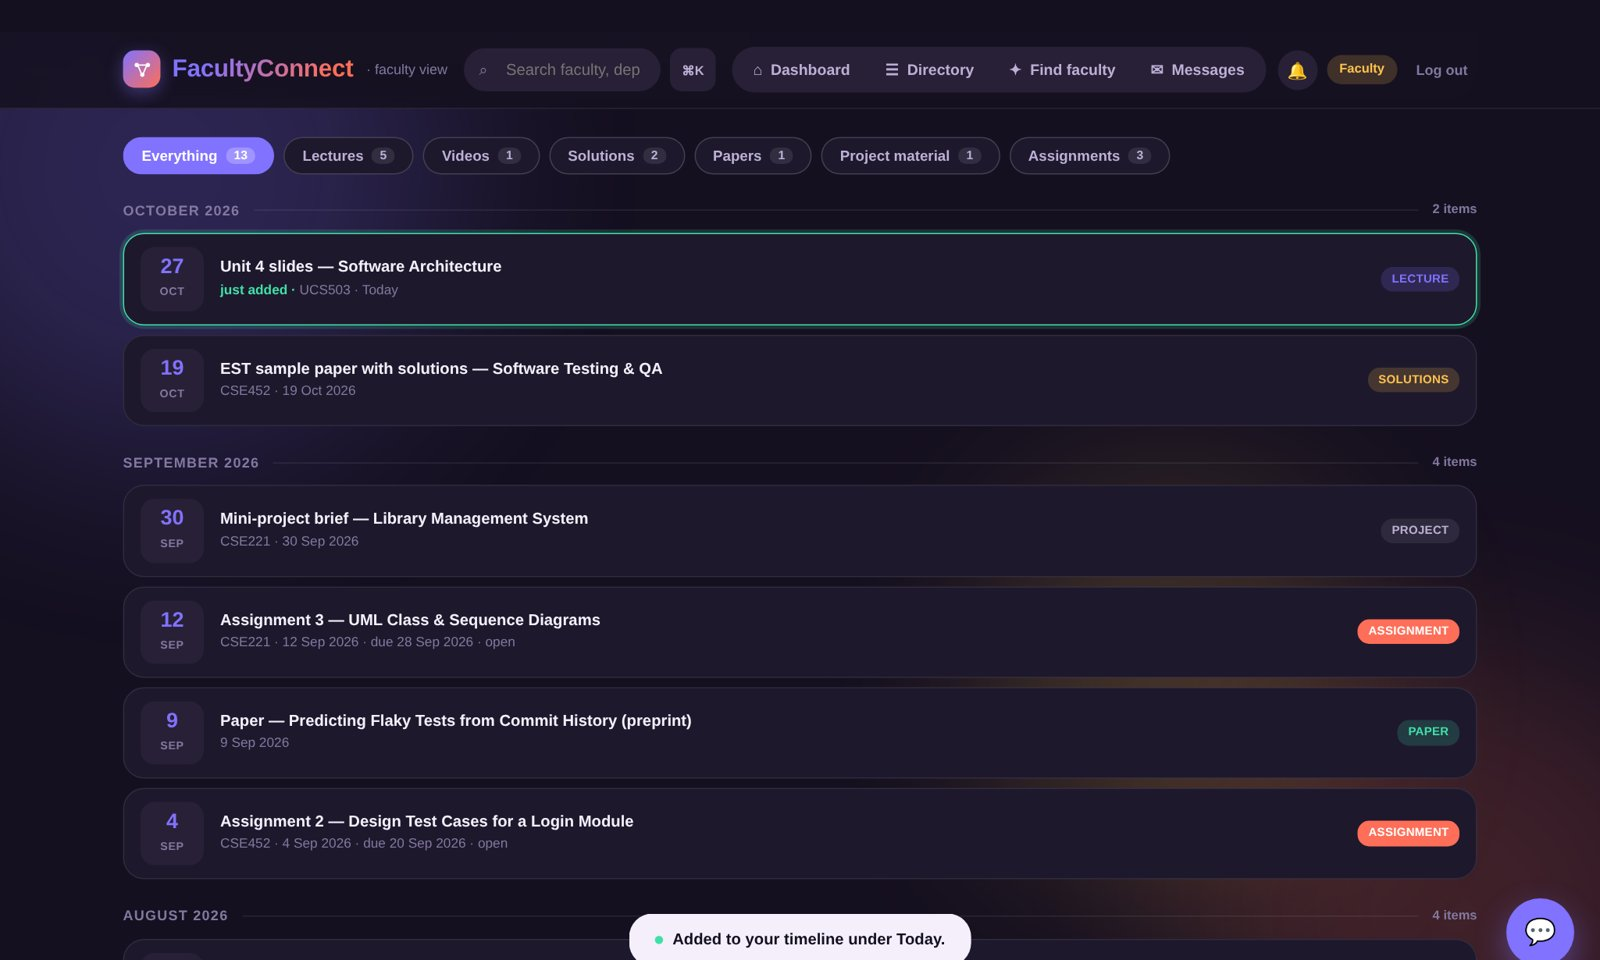
\includegraphics[width=0.84\textwidth]{figures/timeline.jpg}\\[3pt]{\footnotesize (a) All work timeline: newest first, grouped by month, filter by type}\\[14pt]
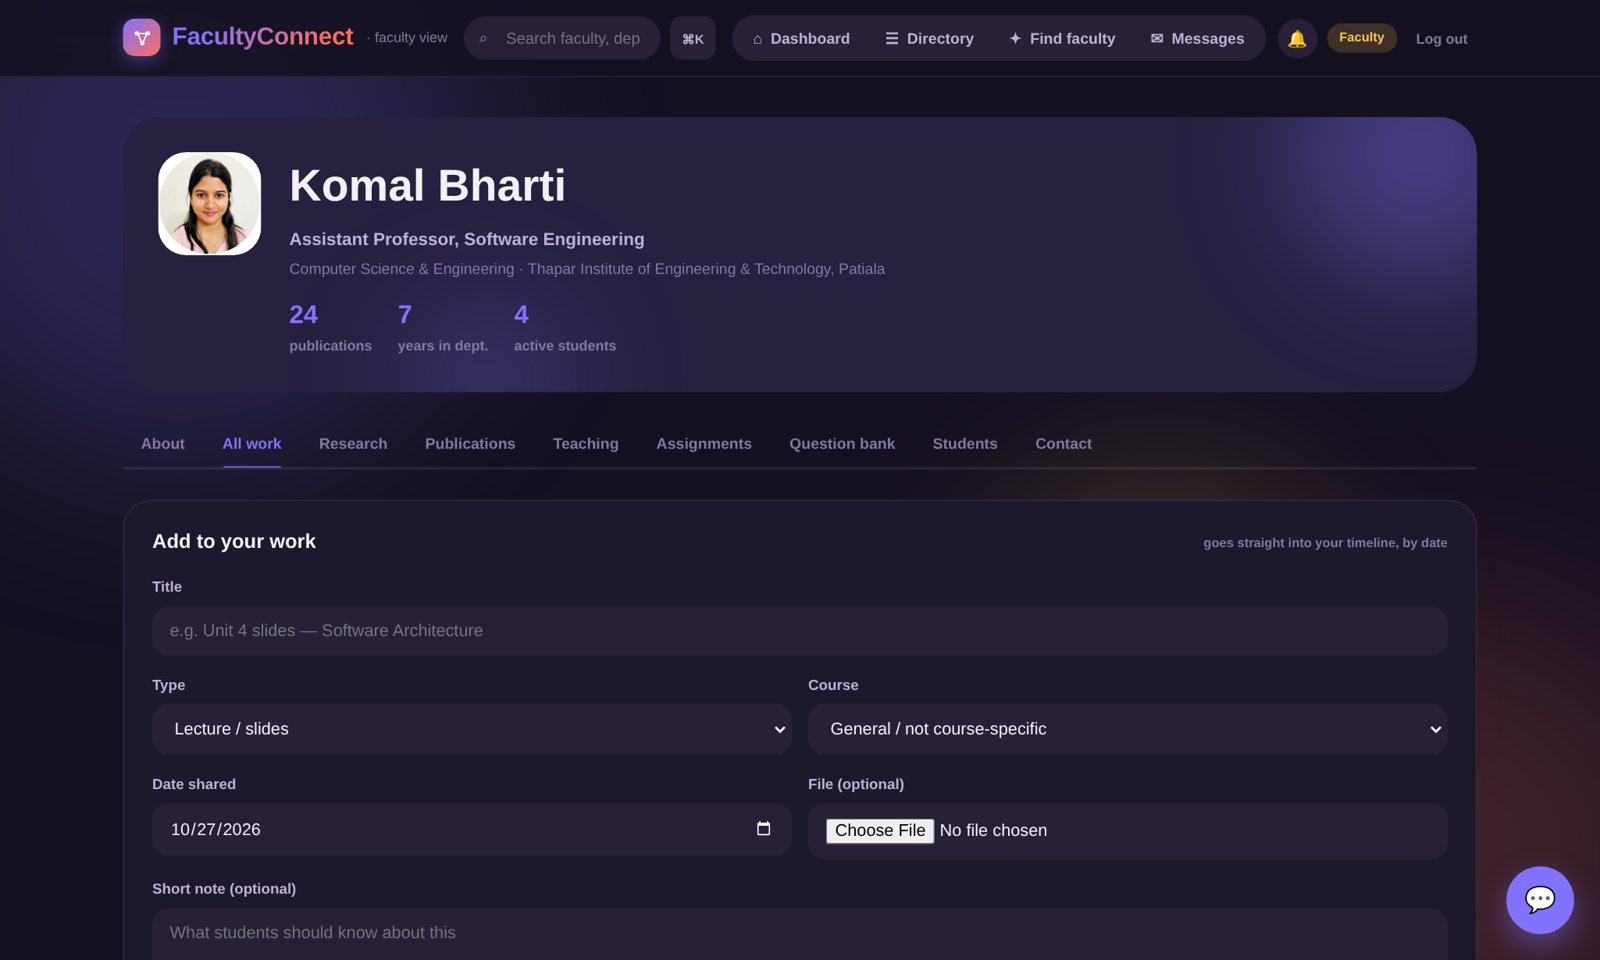
\includegraphics[width=0.84\textwidth]{figures/composer.jpg}\\[3pt]{\footnotesize (b) Faculty adding work, which goes straight into the timeline}
\caption{The unified All work timeline.}
\label{fig:big1}
\end{figure*}

\begin{figure*}[p]
\centering
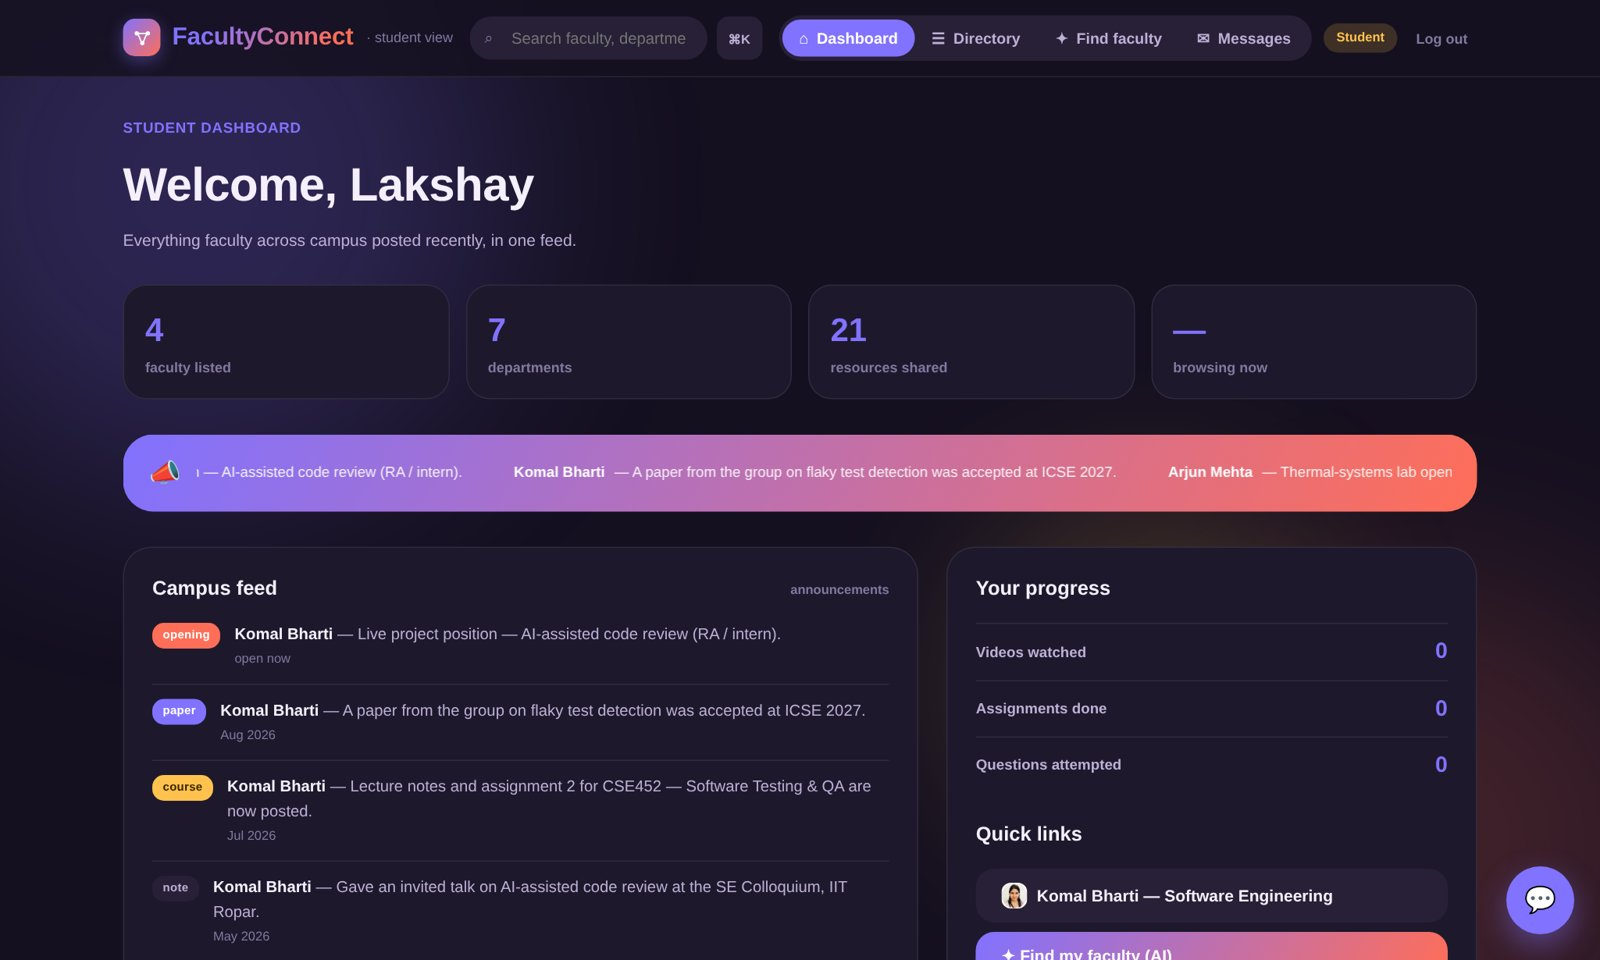
\includegraphics[width=0.84\textwidth]{figures/dashboard-student.jpg}\\[3pt]{\footnotesize (a) Student dashboard: statistics, campus feed, progress}\\[14pt]

\includegraphics[width=0.84\textwidth]{figures/profile.jpg}\\[3pt]{\footnotesize (b) Faculty profile with nine tabs}
\caption{Student dashboard and faculty profile.}
\label{fig:big2}
\end{figure*}

\begin{figure*}[p]
\centering
\begin{minipage}[t]{0.485\textwidth}\centering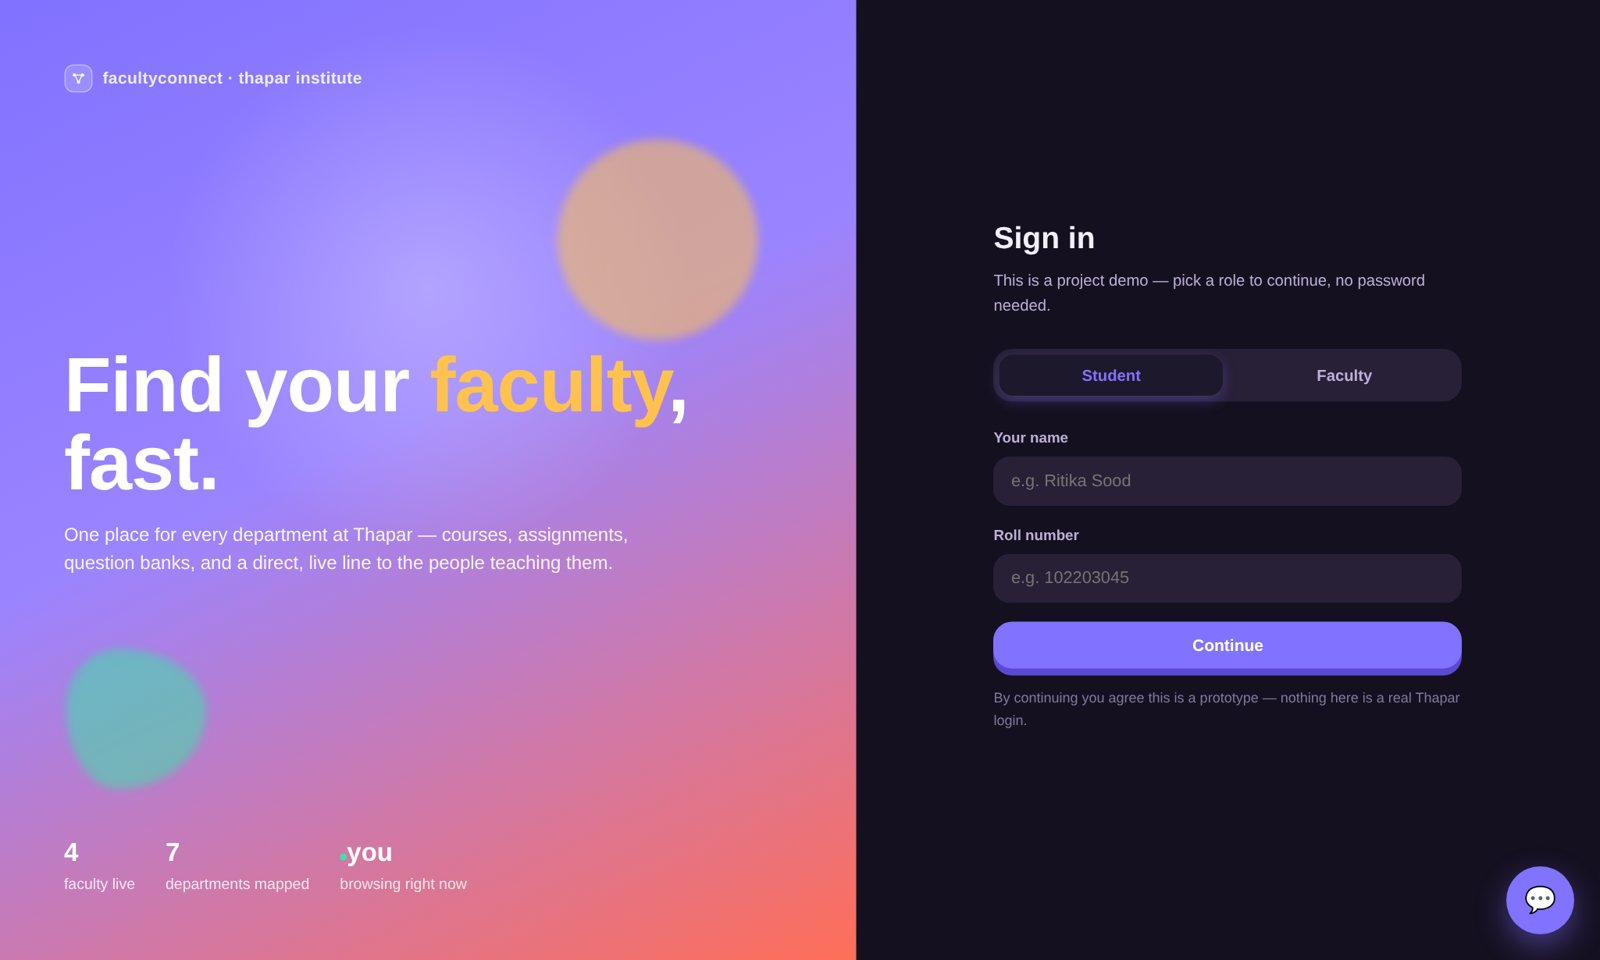
\includegraphics[width=\linewidth]{figures/login.jpg}\\[2pt]{\footnotesize (a) Role-based sign-in}\end{minipage}\hfill
\begin{minipage}[t]{0.485\textwidth}\centering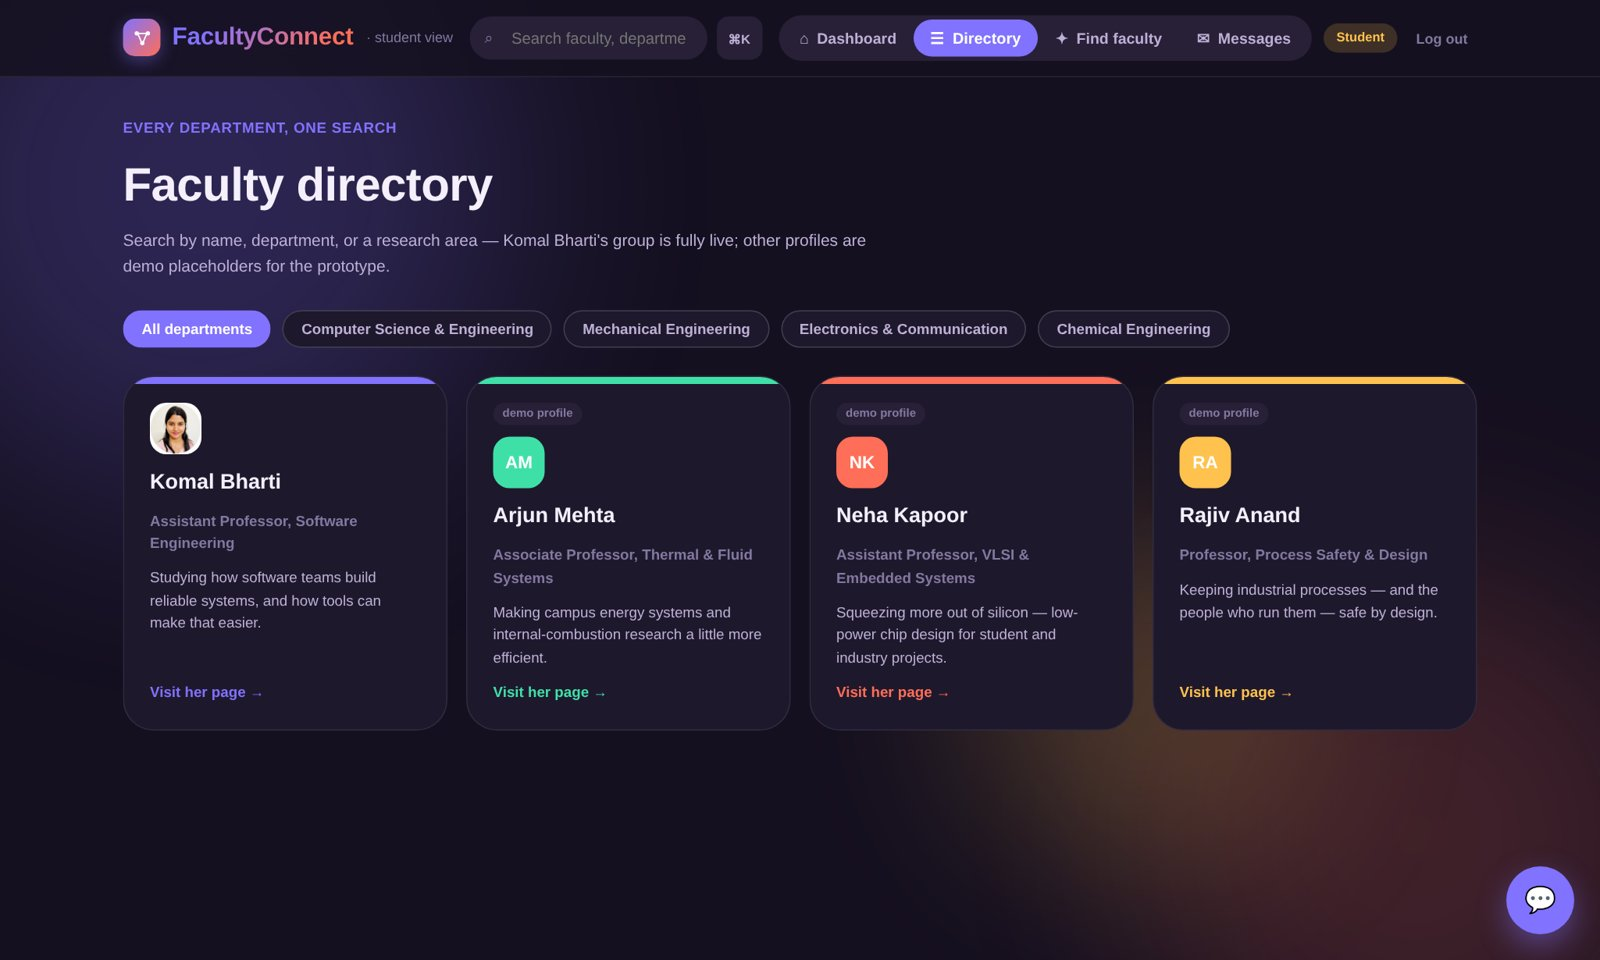
\includegraphics[width=\linewidth]{figures/directory.jpg}\\[2pt]{\footnotesize (b) Faculty directory}\end{minipage}\\[9pt]
\begin{minipage}[t]{0.485\textwidth}\centering
\includegraphics[width=\linewidth]{figures/item-modal.jpg}\\[2pt]{\footnotesize (c) Opening a timeline item}\end{minipage}\hfill
\begin{minipage}[t]{0.485\textwidth}\centering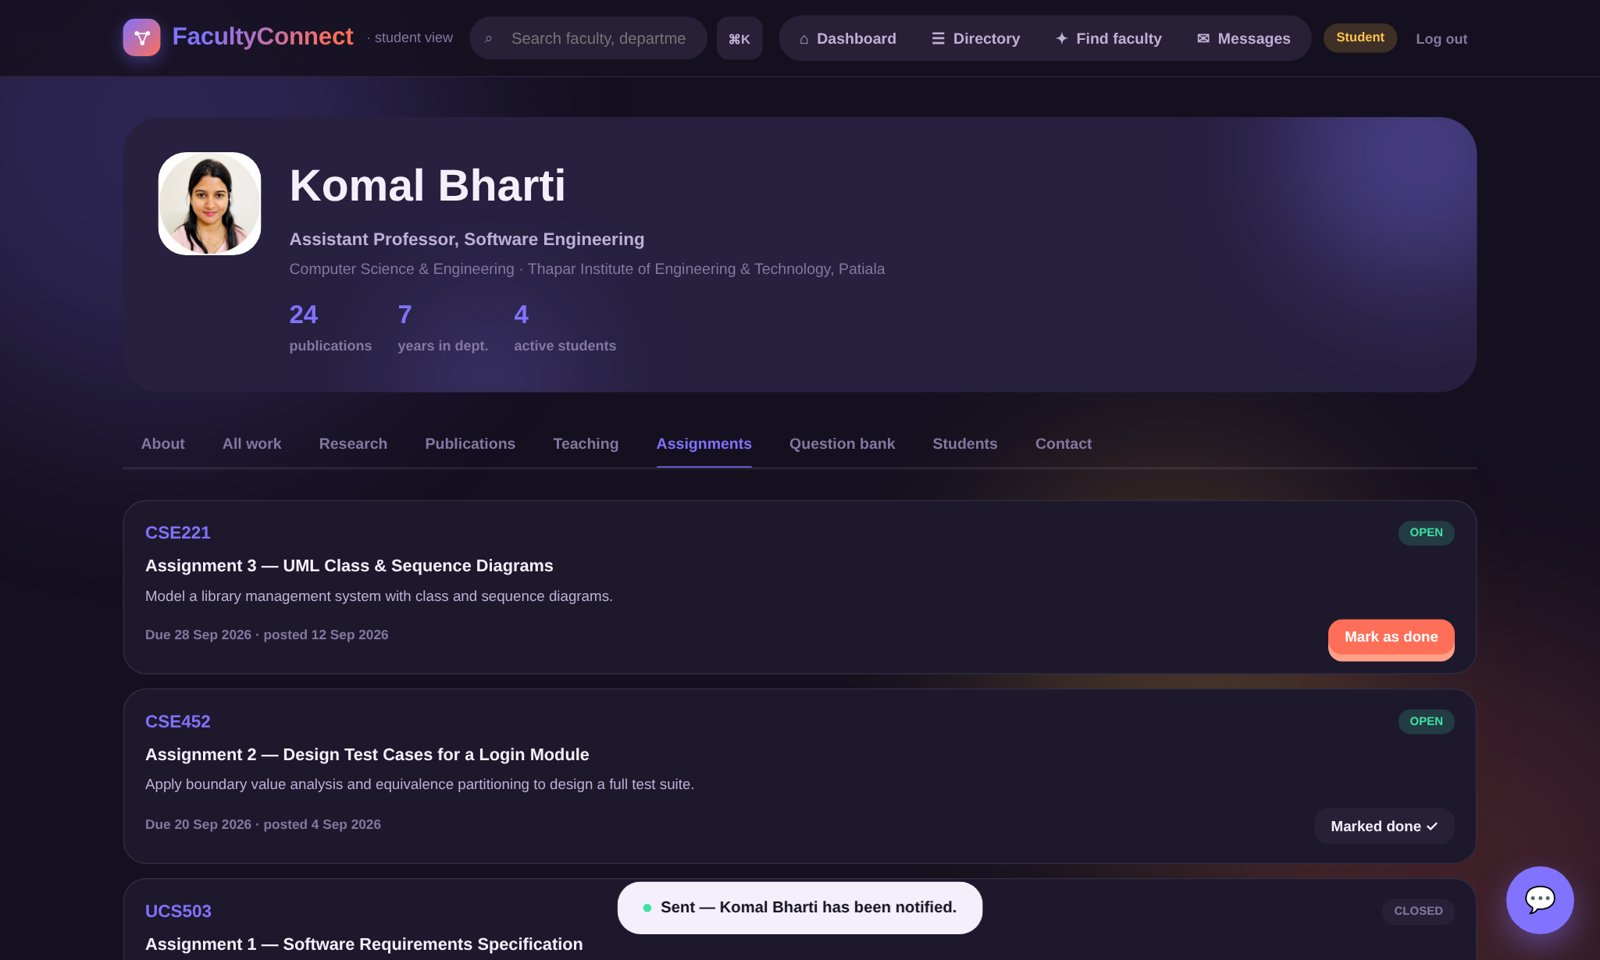
\includegraphics[width=\linewidth]{figures/assignments.jpg}\\[2pt]{\footnotesize (d) Assignments with status}\end{minipage}\\[9pt]
\begin{minipage}[t]{0.485\textwidth}\centering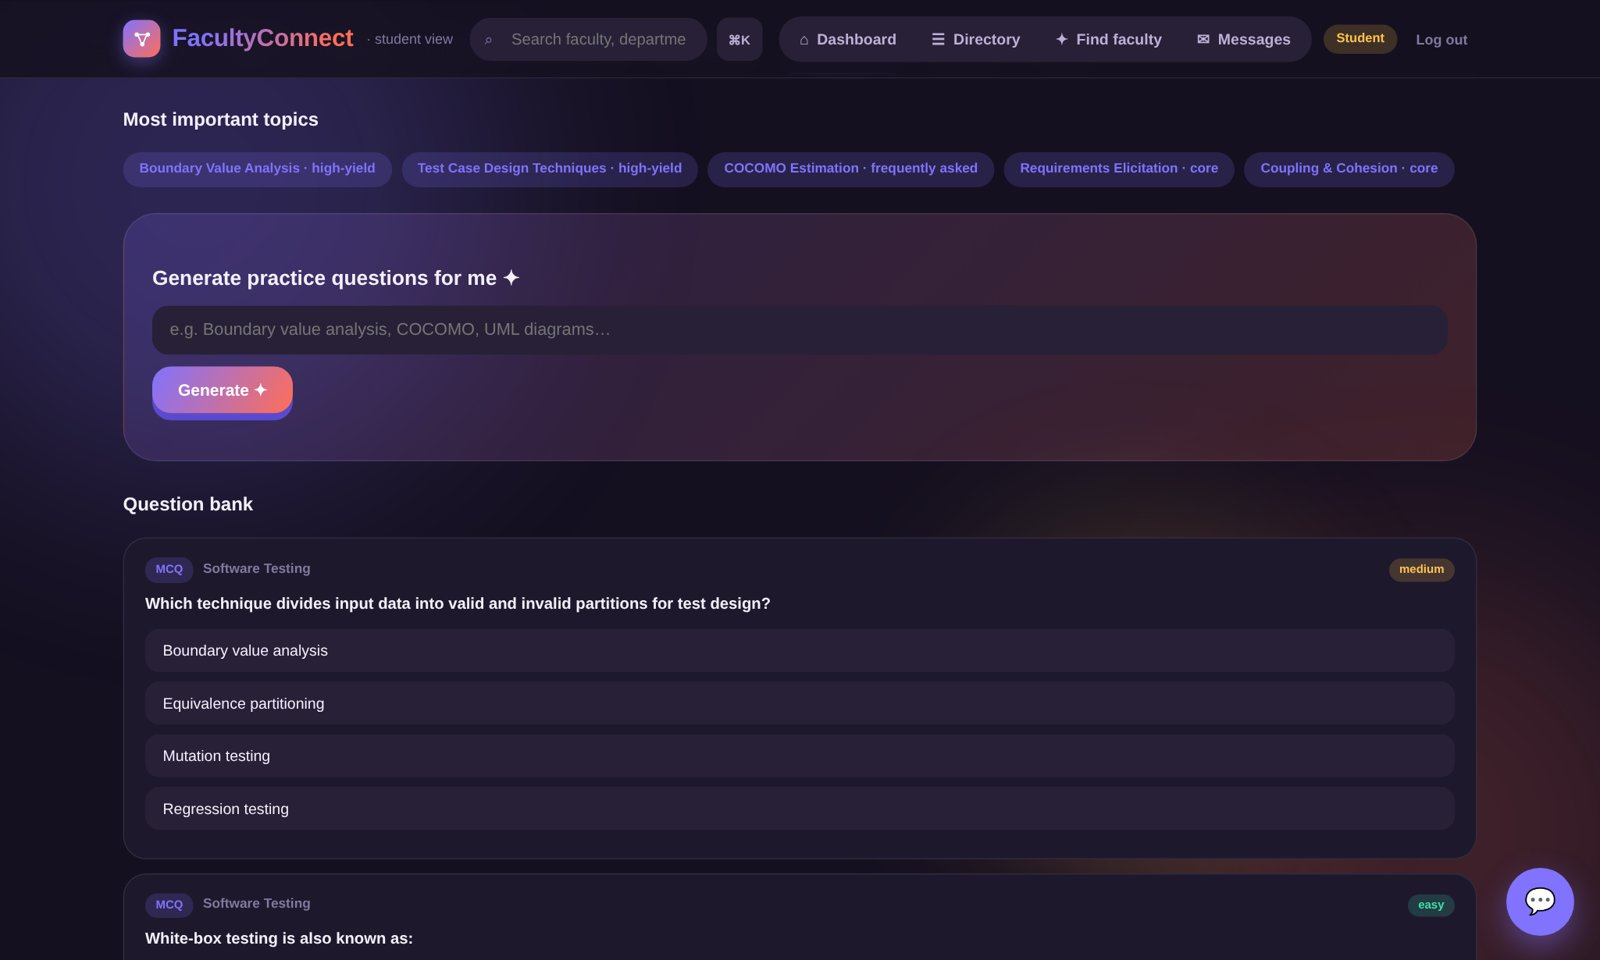
\includegraphics[width=\linewidth]{figures/questionbank.jpg}\\[2pt]{\footnotesize (e) Question bank}\end{minipage}\hfill
\begin{minipage}[t]{0.485\textwidth}\centering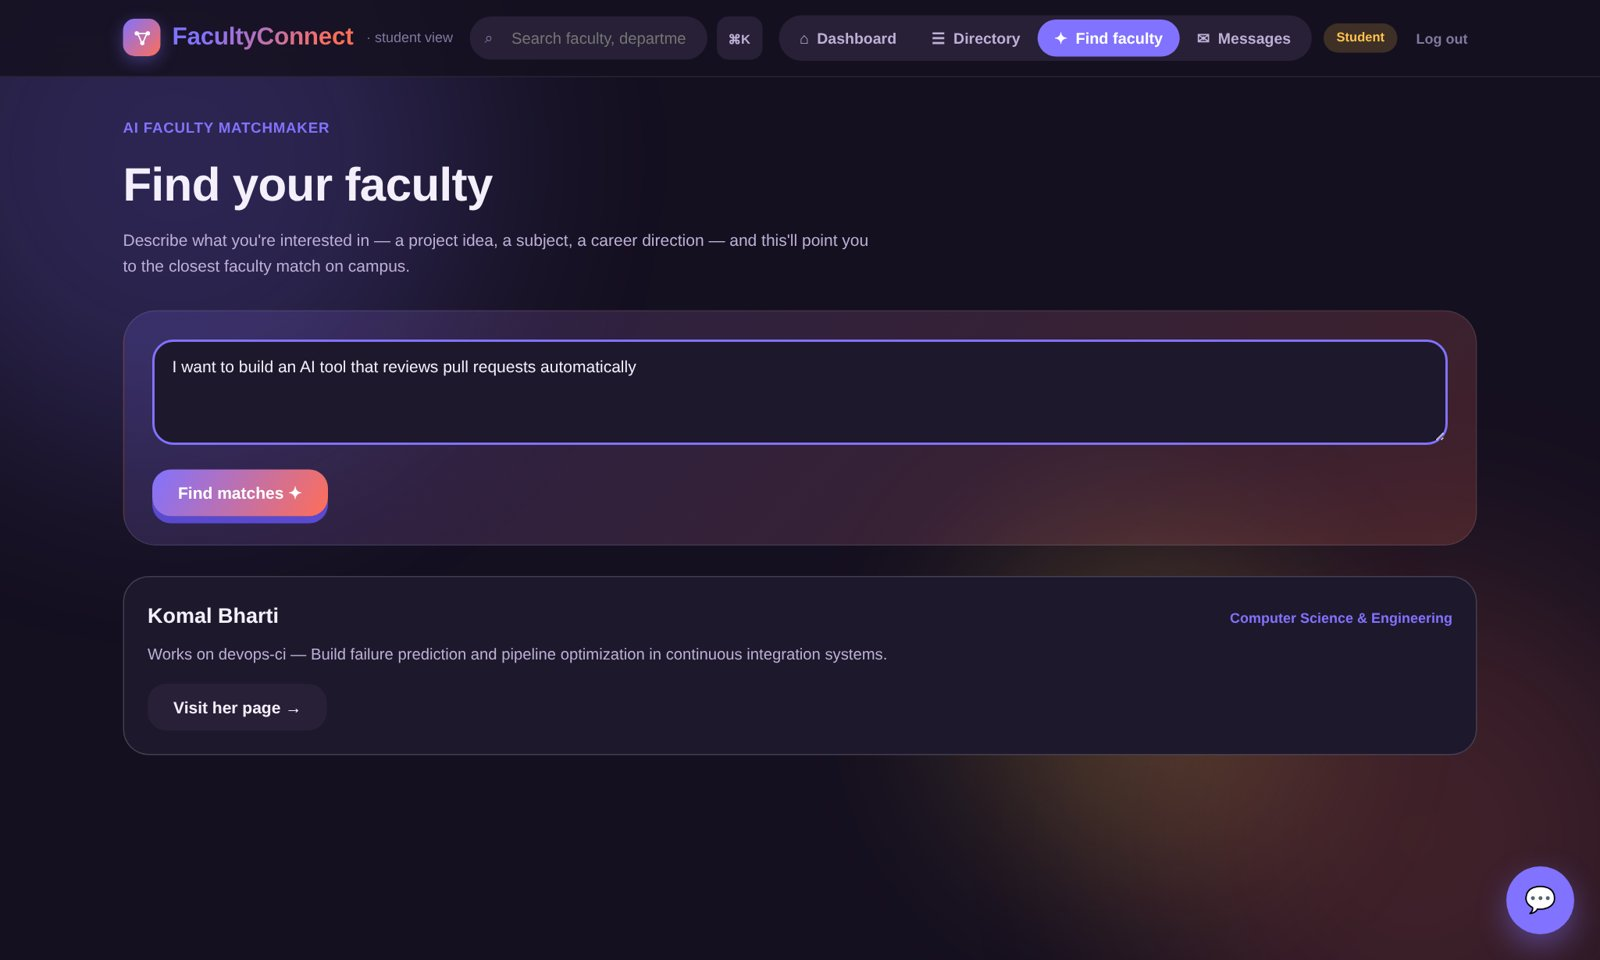
\includegraphics[width=\linewidth]{figures/match.jpg}\\[2pt]{\footnotesize (f) AI faculty recommendation}\end{minipage}\\[9pt]
\begin{minipage}[t]{0.485\textwidth}\centering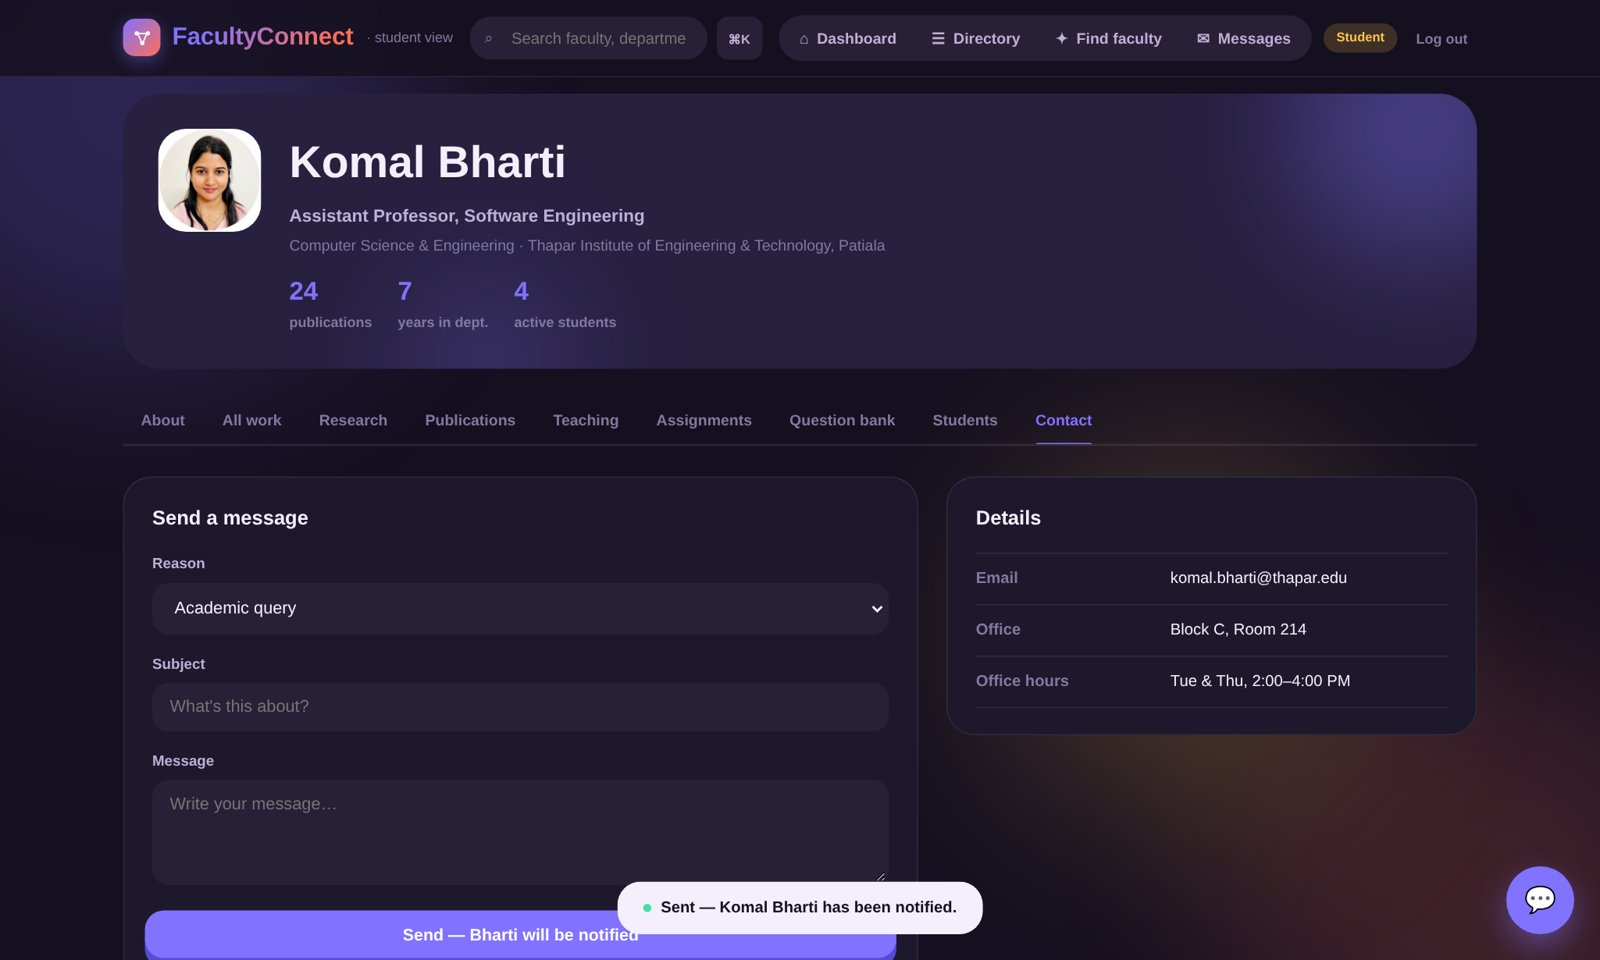
\includegraphics[width=\linewidth]{figures/contact.jpg}\\[2pt]{\footnotesize (g) Structured request}\end{minipage}\hfill
\begin{minipage}[t]{0.485\textwidth}\centering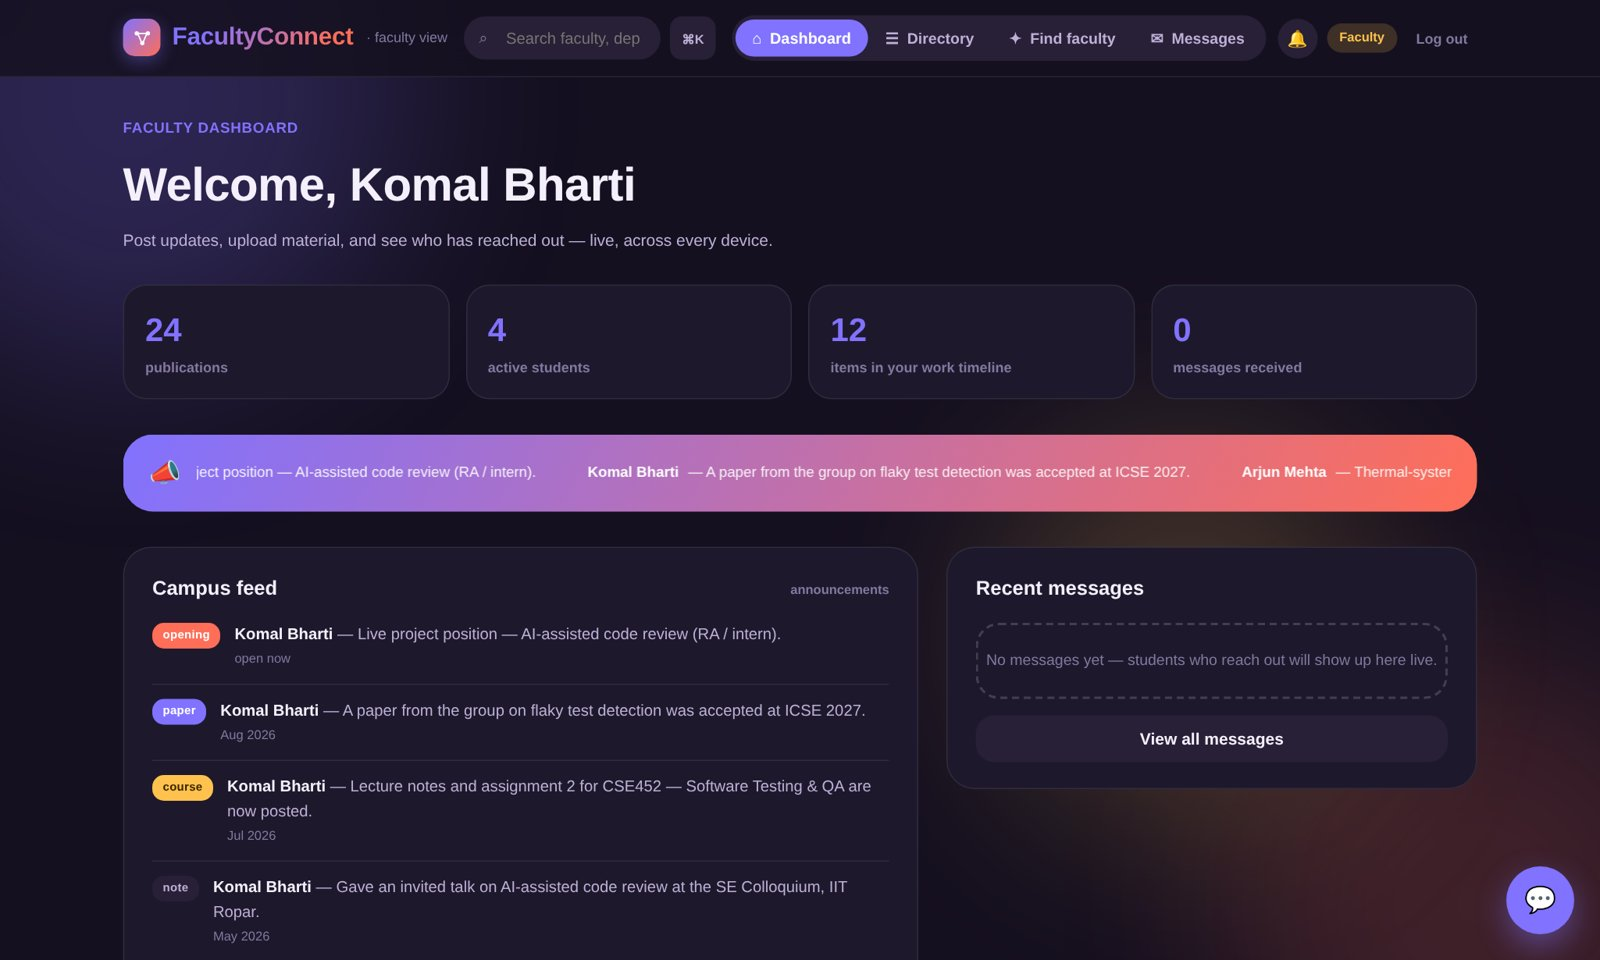
\includegraphics[width=\linewidth]{figures/dashboard-faculty.jpg}\\[2pt]{\footnotesize (h) Faculty dashboard}\end{minipage}
\caption{Other screens of the prototype.}
\label{fig:screens2}
\end{figure*}

\begin{figure*}[!t]
\centering
\begin{minipage}[b]{0.40\textwidth}\centering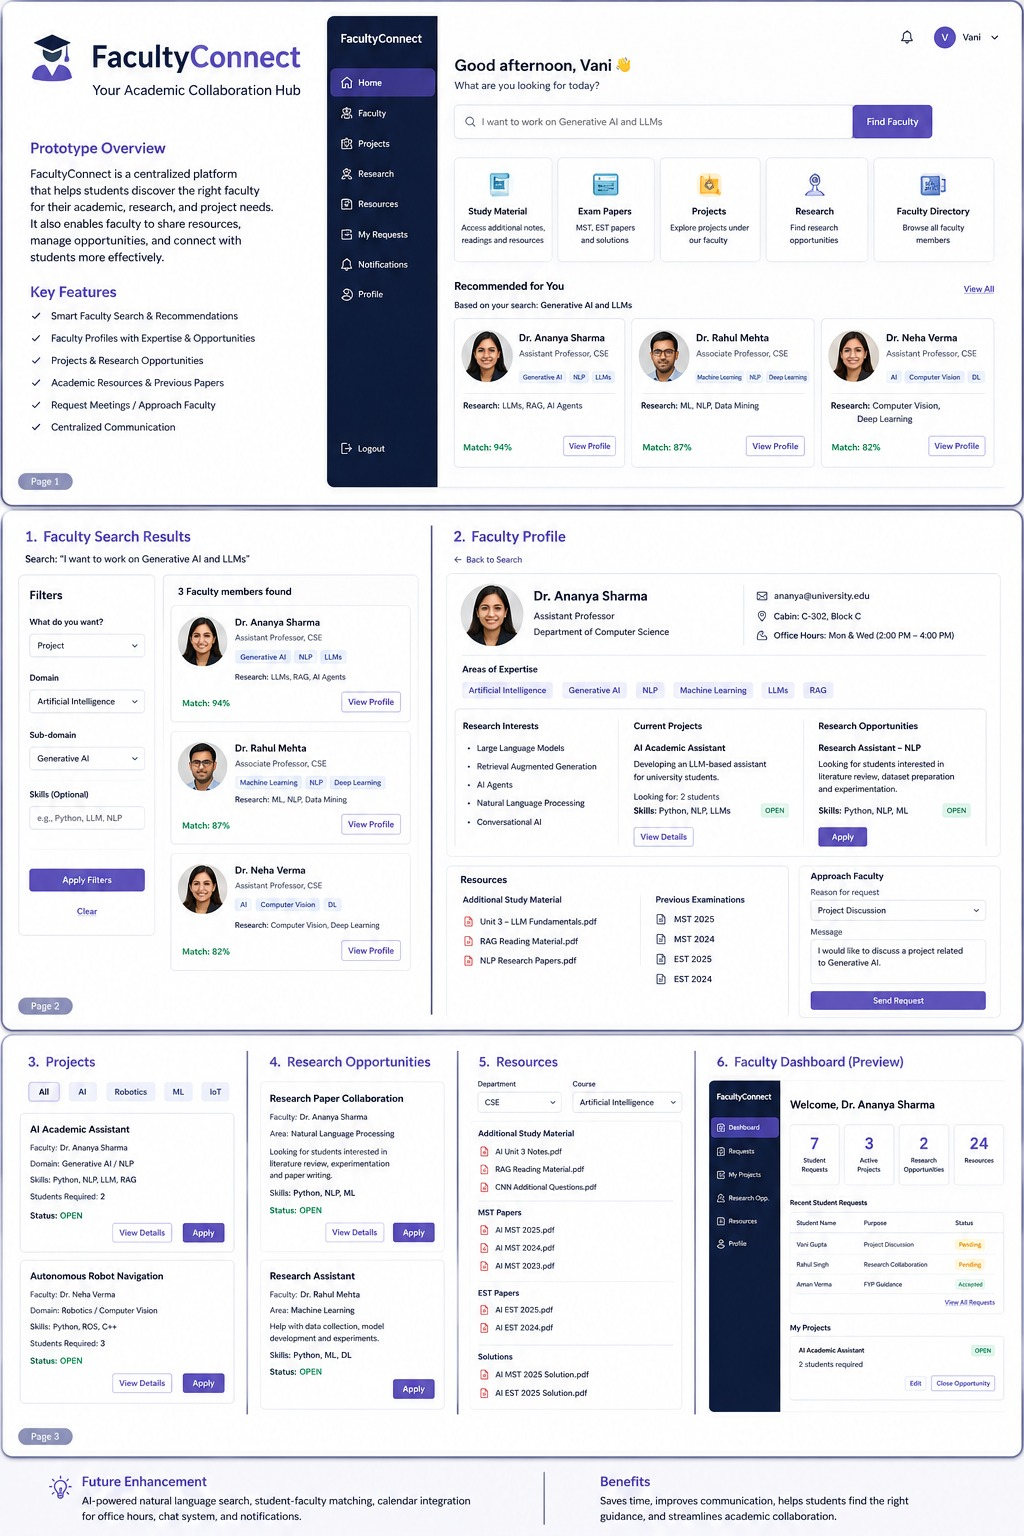
\includegraphics[width=\linewidth]{figures/prototype_mockup.jpg}\\[2pt]{\footnotesize (a) Initial interface concept}\end{minipage}\hfill
\begin{minipage}[b]{0.34\textwidth}\centering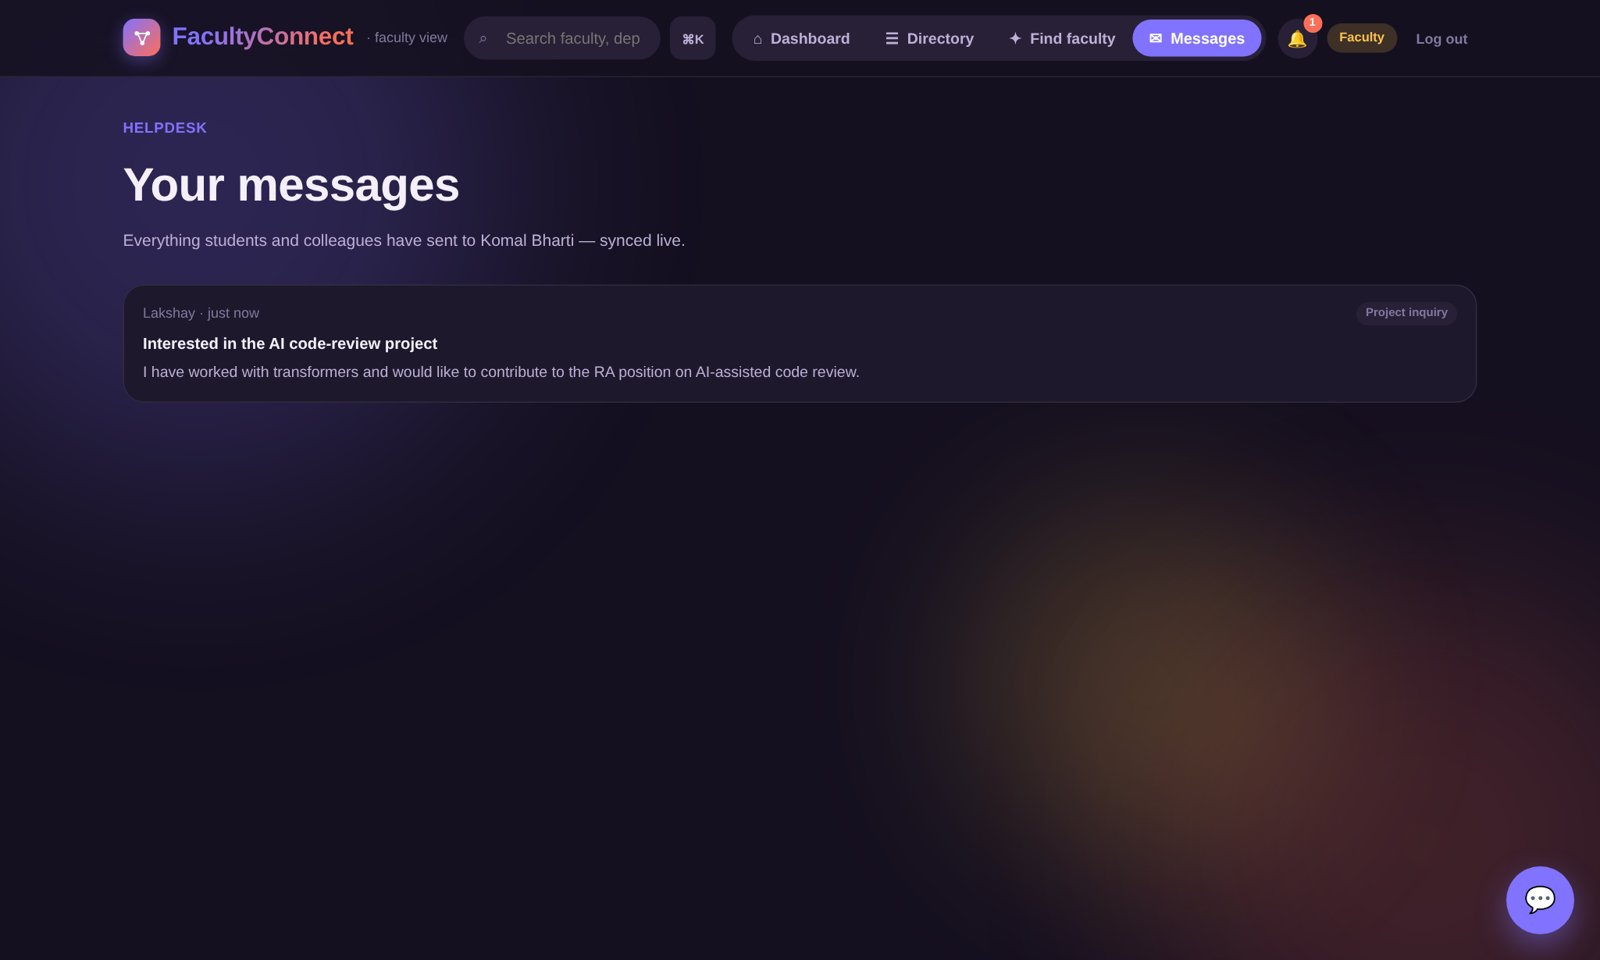
\includegraphics[width=\linewidth,trim=0 330 0 0,clip]{figures/inbox.jpg}\\[2pt]{\footnotesize (b) Faculty inbox receiving the request live}\end{minipage}\hfill
\begin{minipage}[b]{0.22\textwidth}\centering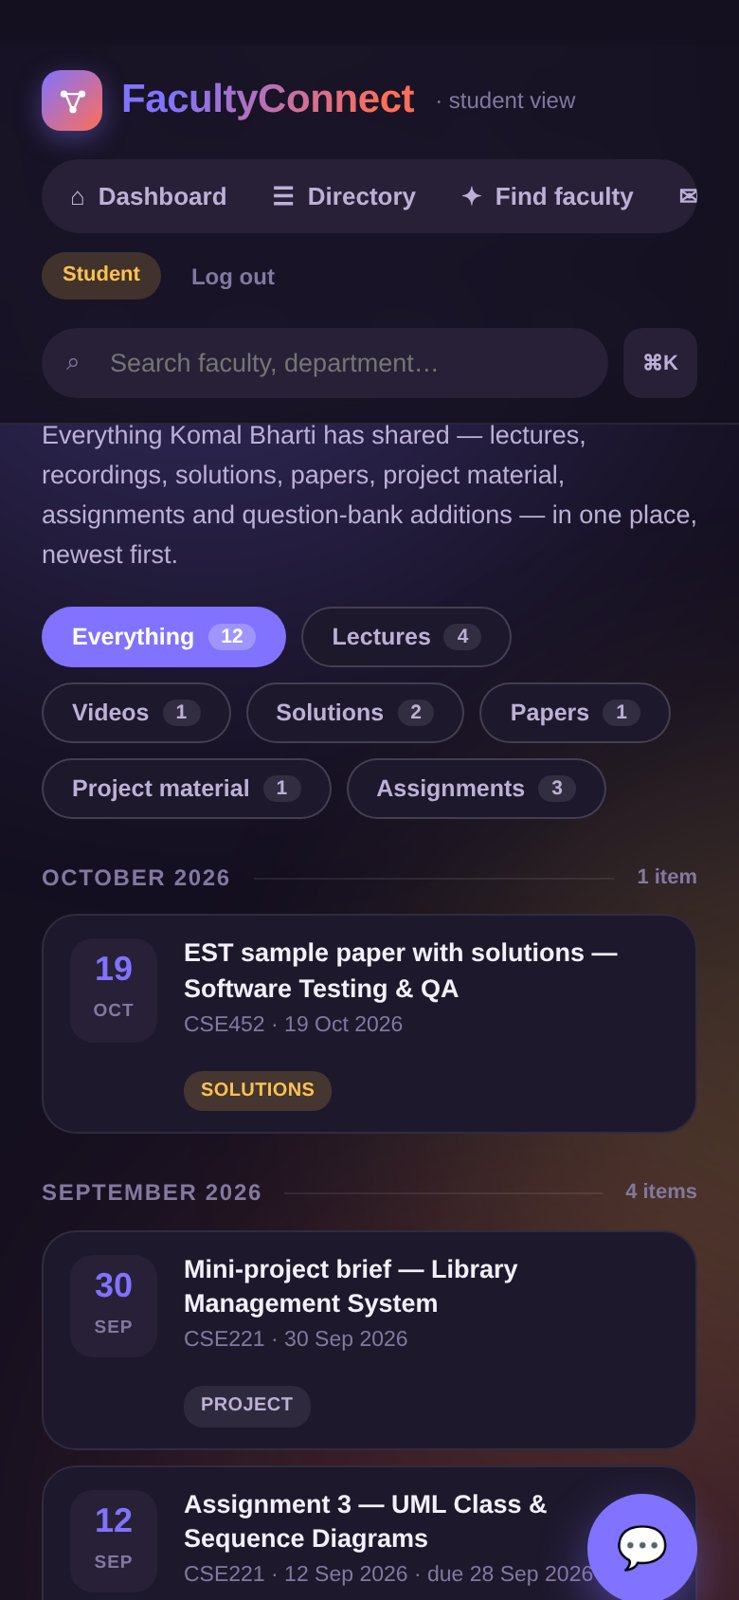
\includegraphics[width=\linewidth]{figures/mobile.jpg}\\[2pt]{\footnotesize (c) Timeline on mobile (390\,px)}\end{minipage}
\caption{Concept, live messaging and mobile view.}
\label{fig:screens3}
\end{figure*}

% =====================================================================
\section{Testing}
The app was tested manually and with automated browser tests (Playwright, headless Chromium) on desktop and mobile widths. Table~\ref{tab:tests} lists the test cases.

\begin{table*}[!t]
\caption{Test Cases}
\label{tab:tests}
\centering\footnotesize
\begin{tabularx}{\textwidth}{@{}l Y Y l@{}}
\toprule
\textbf{ID} & \textbf{Input / action} & \textbf{Expected result} & \textbf{Result}\\
\midrule
T1 & Faculty adds item dated today & Appears first, marked ``just added'' & Pass\\
T2 & Item back-dated to 10 Aug 2026 & Placed between 18 Aug and 4 Aug entries & Pass\\
T3 & Submit with empty title & Blocked; nothing added & Pass\\
T4 & Assignment due 1 Dec 2026 & Shown as \emph{open} & Pass\\
T5 & Assignment due 1 Oct 2026 & Shown as \emph{closed} & Pass\\
T6 & Click \emph{Lectures} filter & Only lectures shown & Pass\\
T7 & Title containing \verb|<script>| & Shown as text, not executed & Pass\\
T8 & Old saved data (``just now'', ``Jul 2026'') & Sorted correctly & Pass\\
T9 & Old link \texttt{\#/faculty/id/lectures} & Opens \emph{All work} tab & Pass\\
T10 & Files of 1.5\,MB and 1.6\,MB (limit 1.5\,MB) & First stored; second keeps name only & Pass\\
T11 & No database or AI available & No errors; local fallback used & Pass\\
T12 & Screen width 360\,px & No horizontal scroll & Pass (after fix)\\
\bottomrule
\end{tabularx}
\end{table*}

\textbf{Bugs fixed:}
\begin{itemize}
  \item Lectures tab crashed on a profile with no lecture data.
  \item Two upload forms shared IDs, so uploads could go to the wrong form.
  \item Toast messages were white text on a white background.
  \item Top navigation overflowed on mobile screens.
\end{itemize}

% =====================================================================
\section{Results}

\begin{table}[!t]
\caption{Before vs. After the Unified Timeline}
\label{tab:effect}
\centering\scriptsize
\begin{tabularx}{\columnwidth}{@{}Y c c@{}}
\toprule
\textbf{Task} & \textbf{Before} & \textbf{After}\\
\midrule
Find latest material from a faculty member & 2--3 tabs & 1 tab\\
Find all solutions shared & 2 lists & 1 click\\
See when an item was shared & not shown & shown\\
Add older work in the right place & no & yes\\
\bottomrule
\end{tabularx}
\end{table}

All core features work in the deployed prototype, which loads as a single 140\,KB page. Table~\ref{tab:effect} shows how the unified timeline simplifies common tasks.

% =====================================================================
\section{Project Plan}

\begin{figure*}[!t]
\centering
\resizebox{0.82\textwidth}{!}{%
\begin{ganttchart}[
  hgrid, vgrid={*1{draw=black!15}},
  x unit=7.5mm, y unit chart=5mm, y unit title=5mm,
  title height=1, bar height=0.55,
  bar/.append style={fill=brand!60,draw=brand},
  milestone/.append style={fill=coral,draw=coral},
  title label font=\scriptsize, bar label font=\scriptsize, milestone label font=\scriptsize]{1}{16}
\gantttitle{Jul}{4}\gantttitle{Aug}{4}\gantttitle{Sep}{4}\gantttitle{Oct}{4}\\
\ganttbar{Requirements \& SRS}{1}{3}\\
\ganttbar{System design}{3}{6}\\
\ganttbar{Profiles \& directory}{5}{8}\\
\ganttbar{Question bank, messaging}{7}{10}\\
\ganttbar{Recommendation, live sync}{9}{12}\\
\ganttmilestone{Vercel deployment}{12}\\
\ganttbar{Unified timeline}{13}{15}\\
\ganttbar{Testing \& report}{14}{16}
\end{ganttchart}}
\caption{Project schedule (July--October 2026).}
\label{fig:gantt}
\end{figure*}

% EDIT the role split below so it matches what each member actually did.
\begin{table}[!t]
\caption{Team Roles}
\label{tab:team}
\centering\scriptsize
\begin{tabularx}{\columnwidth}{@{}l Y@{}}
\toprule
\textbf{Member} & \textbf{Responsibilities}\\
\midrule
Vani Tripathi & Requirements, SRS, UML diagrams, report\\
Agrim Mittal & System design, front end, All work timeline\\
Shriyam Bhardwaj & Recommender, testing, deployment\\
\bottomrule
\end{tabularx}
\end{table}

Fig.~\ref{fig:gantt} shows the schedule and Table~\ref{tab:team} the team roles.

\clearpage
% =====================================================================
\section{Future Scope}
\begin{itemize}
  \item Move to the full React.js + Node.js stack with institute login.
  \item Semantic (embedding-based) faculty matching.
  \item Cloud file storage and administrator console.
  \item Edit/delete timeline items and calendar integration.
  \item Mobile app and push notifications.
\end{itemize}

% =====================================================================
\section{Conclusion}
FacultyConnect brings faculty discovery, shared material, assessments and communication into one platform. The unified \emph{All work} timeline lets students see everything a faculty member has shared, in date order, in one place. The working prototype meets the core requirements and provides a base for a full production system.

% =====================================================================
\begin{thebibliography}{9}
\bibitem{pressman} R.~S. Pressman and B.~R. Maxim, \emph{Software Engineering: A Practitioner's Approach}, 9th~ed. McGraw-Hill, 2020.
\bibitem{sommerville} I.~Sommerville, \emph{Software Engineering}, 10th~ed. Pearson, 2016.
\bibitem{ieee830} \emph{IEEE Recommended Practice for Software Requirements Specifications}, IEEE Std 830-1998.
\bibitem{ricci} F.~Ricci, L.~Rokach, and B.~Shapira, Eds., \emph{Recommender Systems Handbook}, 3rd~ed. Springer, 2022.
\bibitem{playwright} Microsoft, ``Playwright documentation.'' [Online]. Available: \url{https://playwright.dev}
\bibitem{vercel} Vercel Inc., ``Vercel documentation.'' [Online]. Available: \url{https://vercel.com/docs}
\end{thebibliography}

\end{document}
